\documentclass[12pt]{standalone}
\usepackage{tikz}
%\usetikzlibrary{calc, arrows.meta, decorations.pathreplacing}

\begin{document}

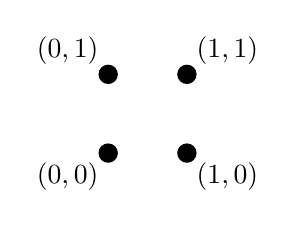
\begin{tikzpicture}[scale=1]
  \fill (0,0) circle[radius=3.5pt];
  \node[below left] at (0,0) {$(0,0)$};

  \fill (0,1) circle[radius=3.5pt];
  \node[above left] at (0,1) {$(0,1)$};

  \fill (1,0) circle[radius=3.5pt];
  \node[below right] at (1,0) {$(1,0)$};

  \fill (1,1) circle[radius=3.5pt];
  \node[above right] at (1,1) {$(1,1)$};
\end{tikzpicture}

\end{document}
